\section{Συνάρτηση Μεταφοράς Κεφαλιού - HRTF} \label{sec:HRTF}


Η συνάρτηση μεταφοράς του κεφαλιού (Head Related Trasnfer Function - HRTF) είναι μια συνάρτηση μεταφοράς, που για μια συγκεκριμένη γωνία πρόσπτωσης, περιγράφει τη μετάδοση του ήχου από ένα ελεύθερο πεδίο (free field) και την επίδραση του κεφαλιού, του λοβού και του θώρακα σε ένα σημείο στο κανάλι του αυτιού (Σχήμα \ref{fig:auditory_system}) ενός ανθρώπου \cite{mller1995head}. Στο πεδίο του χρόνου η HRTF λέγεται κρουστική απόκριση κεφαλιού (Head Related Impulse Response - HRIR). Η HRIR Παρουσιάζει με έναν εύχρηστο και συνοπτικό τρόπο το ILD και ITD μεταξύ των αυτιών καθώς και άλλες φασματικές πληροφορίες \cite{Enzner2013}.

Στην \cite{doi:10.1121/1.415856}, η συνολική ακουστική μεταφορά από μία ακουστική πηγή σε ελεύθερο χώρο έως το τύμπανο ενός ακροατή, χωρίζεται σε τρία κομμάτια ως εξής:

\begin{itemize}
    \item Μεταφορά από ελεύθερο πεδίο στην φραγμένη είσοδο του ακουστικού καναλιού
    \item Μετατροπή της αντίστασης που σχετίζεται με την φραγή του ακουστικού καναλιού
    \item Μεταφορά μέσω του ακουστικού καναλιού
\end{itemize}{}

\subsection{Μέτρηση HRTF}

Ένα σετ HRTF αριστερού και δεξιού αυτιού εξαρτάται από την θέση της πηγής, την θέση του ακροατή, τη θέση του κεφαλιού και του θώρακα και άλλες παραμέτρους. Οι τυπικές διατάξεις μέτρησης, επιτρέπουν τη μεταβολή ενός ή δύο βαθμών ελευθερίας. Στις περισσότερες περιπτώσεις, μεταβάλλεται η γωνία της πηγής, σε σχέση με το κεφάλι και τον θώρακα που έχουν σταθερό προσανατολισμό. Για την αποτελεσματικότερη μέτρηση HRIR και BRIR (βλ. \ref{sec:BRIR}) έχουν κατασκευαστεί βοηθητικά μοτέρ που επιτρέπουν την περιστροφή ή την αλλαγή της κλίσης του κεφαλιού μέσω λογισμικού, με ακρίβεια μέχρι και $0.01^o$. Συνήθως γίνονται μετρήσεις στο διάστημα $\pm90^o$, με τις $0^ο$ να είναι η πηγή ακριβώς μπροστά από τον δέκτη. Στο Σχήμα \ref{fig:typical-HRTF-measurment-setup} φαίνονται δύο τυπικές διατάξεις μέτρησης HRTF. 

\begin{figure}[h]
  \centering
  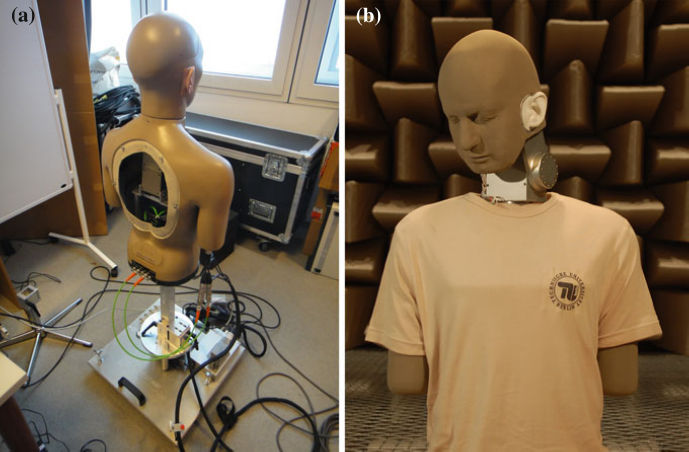
\includegraphics[width=\textwidth]{images/typical-HRTF-measurment-setup.png}
  \caption{Τυπικά σενάρια μέτρησης HRTF: Τροποποιημένο ανδρείκελο KEMAR (a), FABIAN (b)}
  \label{fig:typical-HRTF-measurment-setup}
\end{figure}

\subsection{Υπολογισμός HRTF}

Η επιλογή του σήματος διέγερσης που εκπέμπει η πηγή διαδραματίζει πολύ μεγάλο ρόλο στα αποτελέσματα. Η βέλτιστη διέγερση, εξαρτάται κυρίως από τον αλγόριθμο υπολογισμού της HRIR, αλλά ταυτόχρονα και από το σενάριο μέτρησης (στατικό ή δυναμικό, το περιβάλλον, το υλικό που χρησιμοποιείται κλπ.). Για την επίτευξη ενός υψηλού SNR, το σήμα διέγερσης πρέπει να έχει υψηλή ενέργεια, συγκριτικά με το σύστημα μέτρησης, σε όλη τη συχνοτική περιοχή ενδιαφέροντος. Συχνότερα χρησιμοποιούνται Maximum Length Sequences (MLS), τα οποία είναι περιοδικές ακολουθίες bit που δημιουργούνται από καταχωρητές μετατόπισης γραμμικής ανατροφοδότησης (linear-feedback shift registers) ή απεριοδικά sweep.

Στη συνέχεια, το σήμα αναπαράγεται από το ηχείο-πηγή, και γίνεται συγχρονισμένα η καταγραφή της απόκρισης του αριστερού και δεξιού καναλιού. Η απόκριση συχνότητας προκύπτει από γραμμική αποσυνέλιξη, συνήθως στο πεδίο της συχνότητας. Ένα αποδεκτό SNR για τέτοιου είδους μετρήσεις είναι κάπου ανάμεσα στα 60-90 dB. Μετρήσεις HRTF, πλέον γίνονται και σε ανθρώπους, όχι μόνο σε ανδρείκελα, με ειδικά κατασκευασμένα ακουστικά το περίβλημα των οποίων τυπώνεται με 3Δ εκτυπωτές. 

\subsection{Βάσεις δεδομένων HRTF}

Οι HRTF είναι ένα αναπόσπαστο κομμάτι της τεχνολογίας αμφιωτικής ακοής και ακρόασης. Από την άλλη, η μέτρηση των HRTF είναι ένα δύσκολο και ευαίσθητο εργαστηριακό αντικείμενο. Συνήθως απαιτείται ένας ανηχοϊκός θάλαμος για τη μέτρηση των HRTF, και επιπλέον αρκετός χρόνος από την πλευρά του χειριστή του πειράματος αλλά και του υποκειμένου μέτρησης, ώστε να ολοκληρωθούν οι μετρήσεις με ικανοποιητικό βαθμό χωρικής ανάλυσης. Απαιτούνται ένα ή περισσότερα ηχεία, ακουστικά in-ear, και λογισμικό αναπαραγωγής και καταγραφής ήχου. 

Υπάρχουν αρκετά τέτοια συστήματα, αλλά είναι σαφές πως δεν είναι φορητά. Ως αποτέλεσμα, πολλοί οργανισμοί έχουν επιλέξει να παρέχουν τις μετρήσεις ως δημόσια διαθέσιμες βάσεις δεδομένων στην κοινότητα. Παρακάτω αναφέρονται κάποιες από αυτές. Εκτός αν αναφέρεται διαφορετικά, οι κρουστικές αποκρίσεις παρέχονται με συχνότητα δειγματοληψίας $F_s = 44.1 kHz$.

\begin{itemize}
   \item KEMAR - βάση δεδομένων HRTF από το MIT-Media-Lab \cite{Gardner1995}: Η πρώιμη αυτή βάση δεδομένων είναι ακόμα ιδιαίτερα δημοφιλής, χρησιμοποιώντας το Knowles-Electronics Mannequin for Acoustic Research (KEMAR), αναπαριστά μια εκτενή καταγραφή HRTF. Συνολικά, δειγματοληπτούνται 710 διαφορετικές θέσης, για ανύψωση από $-40^o$ μέχρι $+90^o$ με χωρική ανάλυση $10^o$ στον κάθετο άξονα και περίπου $5^o$ στον οριζόντιο, για απόσταση περίπου 1.4 m μεταξύ του ηχείου και του KEMAR.
   
   \item AUDIS - Ο κατάλογος AUDIS ανθρωπίνων HRTF: Στο γενικό πλαίσιο της Ε.Ε., το project Auditory Displays (AUDIS) \cite{Blauert_1998}, το οποίο βασίστηκε σε μεγάλο βαθμό στην αμφιωτική τεχνολογία και αξιόπιστες HRTF ανθρώπων, πραγματοποιήθηκε ένα ειδικό πρόγραμμα συλλογής HRTF. Εδώ οι συνθήκες μετρήσεων είναι: 2.4 m από το ηχείο, ανάλυση $10^o$ στον κάθετο άξονα από $-10^o$ μέχρι $+90^o$, και ανάλυση $15^o$ στον οριζόντιο άξονα. Οι συνολικές μετρήσεις περιλαμβάνουν 122 κατευθύνσεις για 20 ανθρώπους. Τέθηκε επίσης ένα σύνολο \textit{Golden Rules} για μετρήσεις HRTF.
   
   \item CIPIC - βάση δεδομένων HRTF του εργαστηρίου CIPIC \cite{AlgaziOct.21242001}: Η βάση δεδομένων, περιέχει HRTF μετρημένες με υψηλή χωρική ανάλυση, για περισσότερους από 90 ανθρώπους, με 45 αυτών να είναι δημόσια διαθέσιμοι, συμπεριλαμβανομένου του KEMAR, με μεγάλο και μικρό λοβό. Η χωρική ανάλυση είναι $5^o$ στον κάθετο αλλά και στον οριζόντιο άξονα. Προκύπτουν έτσι 1250 σημεία στην ακουστική σφαίρα 1m, όπου ήταν η απόσταση του ηχείου. Παρέχονται επίσης ανθρωπομετρικά χαρακτηριστικά για κάθε υποκείμενο μέτρησης, καθώς και βοηθητικές συναρτήσεις για το περιβάλλον MATLAB.
   
   \item LISTEN - η βάση δεδομένων HRTF IRCAM: Αναπτηγμένη σε πρότζεκτ της Ε.Ε., περιέχει μετρήσεις HRTF με για  ανύψωση από $-45^o$ μέχρι $+90^o$ με χωρική ανάλυση $5^o$ και περίπου $15^o$ ανάλυση στον οριζόντιο άξονα. Συνολικά μετριούνται 187 θέσεις. Παρέχονται οι μετρήσεις HRTF, προαιρετική διόρθωση diffuse-field και μορφολογικά δεδομένα. Τα δεδομένα που μετρήθηκαν για 50 ανθρώπους είναι διαθέσιμα online\footnote{http://recherche.ircam.fr/equipes/salles/listen/index.html}.
   
   \item ARI - Βάση δεδομένων του Acoustics-Research-Institute: Περιέχει HRTF υψηλής ανάλυσης για πάνω από 70 ανθρώπους. Μετρήθηκαν 1550 θέσεις για κάθε ακροατή, με $2.5^o$ ανάλυση στον οριζόντιο άξονα για γωνίες από $0^o - 359^o$, και ανυψώσεις από $-30^o$ έως $+80^o$. Τα δεδομένα μπορούν να βρεθούν στον σύνδεσμο\footnote{http://www.kfs.oeaw.ac.at/content/view/608/606}.
   
   \item FIU - Βάση δεδομένων HRTF του Florida-International-Univ. DSP-Lab: Μετρήθηκαν 15 διαφορετικά άτομα, για δώδεκα διαφορετικές γωνίες στον οριζόντιο άξονα και έξι στον κάθετο. Παρέχονται 3-Δ εικόνες των λοβών κάθε ατόμου, και ανθρωπομετρικά χαρακτηριστικά. Χρησιμοποιήθηκε συχνότητα δειγματοληψίας $F_s = 96 kHz$ και είναι διαθέσιμη στον σύνδεσμο\footnote{http://dsp.eng.fiu.edu/HRTFDB}.
\end{itemize}